% ------------------------------------------------------------------------
% NIT Trichy Synopsis Template (MS/PhD)
% Revised by: Shashank Singh, M.S./EEE/(2016-19)
% ------------------------------------------------------------------------
\documentclass[12pt,a4paper, twoside]{report}
\usepackage[labelfont=bf,textfont=bf,labelsep=space,figurename=Fig.]{caption}
\usepackage[round,authoryear]{natbib}
\usepackage[subfigure]{tocloft}
\usepackage{subfig}
\usepackage{etoolbox}
\usepackage[centertags]{amsmath}
\usepackage{amsfonts,amsmath,latexsym,amssymb,amsthm,mathrsfs,amsbsy}
\usepackage{enumerate,tabularx,longtable,multirow,array}
\usepackage{varioref,amscd,verbatim,calc}
\usepackage{algorithm,algpseudocode}
\usepackage{pdfpages,mathptmx,anysize}
\usepackage{newlfont,setspace,titlesec,lipsum}
\usepackage[usenames,dvipsnames]{pstricks}
\usepackage{pstricks,graphicx,epsfig}
\usepackage{makeidx}
\usepackage[shortlabels]{enumitem}
\makeindex
\usepackage[usenames,dvipsnames]{pstricks}
\usepackage{pstricks,graphicx,epsfig}
\usepackage{pst-grad} % For gradients
\usepackage{pst-plot}
\usepackage{indentfirst}
\usepackage{titlesec}
\hyphenpenalty=5000
\titleformat{\chapter}[display]
{\centering\normalsize\bfseries}% instead of \Large you can use the
  {\MakeUppercase{\chaptertitlename}\ \thechapter}{14pt}
  {\normalsize}% change according to your needs

%\usepackage[showframe]{geometry} %Use this to check margin boundaries.
% If using this, comment the next command i.e. %\usepackage{geometry}
\usepackage{geometry}
\geometry{a4paper, top=25mm,left=38mm, right=25mm, bottom=25mm}

\renewcommand{\cftsecleader}{\bfseries\cftdotfill{\cftdotsep}}
\newcolumntype{M}[1]{>{\centering\arraybackslash}m{#1}}
\newcolumntype{P}[1]{>{\centering\arraybackslash}p{#1}}

\makeatletter
\renewcommand*{\l@part}[2]{%
\par\addvspace{\topsep}
\setlength\@tempdima{2.3em}%
\noindent\hspace*{1.5em}\textbf{#1}\par}
\makeatother

\renewcommand*\cftchappresnum{\normalsize\textbf{CHAPTER}~}
\settowidth{\cftchapnumwidth}{\cftchappresnum}
\renewcommand{\cftchapaftersnumb}{\qquad}

\renewcommand{\thesection}{\arabic-{section}}
\renewcommand{\thesection}{\normalsize\arabic{section}}

\renewcommand{\thesubsection}{\normalsize\arabic{section}.\arabic{subsection}}
\renewcommand{\thesubsubsection}{\arabic{section}.\arabic{subsection}.\arabic{subsubsection}}

\titleformat*{\section}{\normalsize\bfseries}
\titleformat*{\subsection}{\normalsize\bfseries}

\newcounter{bibcount}
\makeatletter
\patchcmd{\@lbibitem}{\item[}{\item[\hfil\stepcounter{bibcount}{\thebibcount.}}{}{}
\setlength{\bibhang}{2\parindent}
\renewcommand\NAT@bibsetup%
   [1]{\setlength{\leftmargin}{\bibhang}\setlength{\itemindent}{-\parindent}%
       \setlength{\itemsep}{\bibsep}\setlength{\parsep}{\z@}}
\makeatother

\setlength{\parindent}{3em}
\setlength{\parskip}{1em}

\titlespacing*{\section}{-5pt}{0\baselineskip}{0\baselineskip}

\titlespacing*{\subsection}{-5pt}{0\baselineskip}{0\baselineskip}

\setlist[itemize,enumerate]{noitemsep, topsep=-0.5cm}

%\onehalfspacing

\begin{document}
\thispagestyle{empty}
\setboolean{@twoside}{false}
% This is the title page of Synopsis
% Do not compile/run this file directly
% Rather call this file from Synopsis.tex file
% While printing, print this page separately
% Please start back to back printing from page 1, not from this page (title page). 
\begin{titlepage}
\begin{center}
\thispagestyle{empty}
\large
\textbf{SYNOPSIS OF}\\
\bigskip
\large{\textbf{Insert Thesis Title Here}}
\\
\bigskip \bigskip \bigskip \bigskip  
\large
\textbf {A THESIS}\\
\emph{to be submitted by}\\
\bigskip \bigskip \bigskip \bigskip
\textbf{Name}\\
\textbf{(Roll Number)}
\\
\bigskip \bigskip \bigskip \bigskip
\emph{for the award of the degree}\\ \bigskip \bigskip
\emph{of}\\
\bigskip \bigskip
%Course Name: MASTER OF SCIENCE (BY RESEARCH)
%Course Name: DOCTOR OF PHILOSOPHY
\textbf{MASTER OF SCIENCE (BY RESEARCH)}\\

\bigskip \bigskip \bigskip \bigskip \bigskip  
\centering


\includegraphics[width=1.25in, height=1.25in]{NITT} %Specify NITT Logo file name

\bigskip \bigskip
\normalsize
\large\textbf{DEPARTMENT OF}\\
\large\textbf{ELECTRICAL AND ELECTRONICS ENGINEERING}\\ %Specify Department
\large\textbf{NATIONAL INSTITUTE OF TECHNOLOGY}\\
\large\textbf{TIRUCHIRAPPALLI -- 620015}\\
\vspace{0.20in}
\large\textbf{APRIL 2019} %Specify Month and Year of Synopsis to be submitted
\end{center}
\end{titlepage} 
\spacing{1.3}
\newpage
\setboolean{@twoside}{true}
\section{INTRODUCTION}
Introduction goes here, wherein outline briefly the technological / engineering / scientific / Socioeconomic relevance or significance of the research work is being reported. One sample paragraph is given below.

Electrical power system is one of the most complex and crucial technical innovations of mankind. A legacy power system hosts generation, transmission, distribution and consumption infrastructure, wherein large power plants pump power into the grid and try to keep a balance between generation and demand at all times. Smart grid (SG) is bringing a paradigm shift in the structure of power systems through information and communication technology (ICT), smart computational algorithms, consumers' participation, and trading infrastructure for local renewable generation [\cite{fang2012}]. 

\section{MOTIVATION}
Trace to the pint, the developments in the area, to emphasize the current status and importance of the research problem identified. Sample text is given below.

The advancements in ICT and Internet of Things (IoT) will transcend the limitations of the legacy grid and propel it beyond singularity, that could bridge the gap between the consumers and the grid [\cite{collier2017}]. 

\section{OBJECTIVES AND SCOPE}

\noindent The objectives of the present research work are as follows:

\begin{enumerate}[itemsep=0.2cm,topsep=1pt,parsep=0pt,partopsep=0pt]
\item First Novel Point
\begin{itemize}[itemsep=0cm,topsep=2pt]
\item supportive statements;
\item benefits;
\end{itemize}
\item Second Novel Point
\begin{itemize}[itemsep=0cm,topsep=2pt]
\item supportive statements;
\item benefits;
\end{itemize}

\end{enumerate}

The scope of the present research work adopts a steady state modeling of household appliances from [\cite{arun2017}]. Replace existing sample paragraphs with your paragraphs.

\section{DESCRIPTION OF THE RESEARCH WORK}
Give brief, but sufficient, details regarding:

\subsection{The research problems}
Sample Text.

\subsection{Solution methodologies}
Sample Text.

\subsection{Interpretation of the results / output}
Sample Text and Sample equation.
\begin{equation}
\left(\alpha,\beta,\gamma, T^{set},\Delta T \right)=\left\{ \begin{matrix}
   \left( \text{0,0,0,0,0} \right) & if  \\
   \left( \text{0,0,0,1,1} \right) & if  \\
   \left( \text{1,1,1,0,0} \right) & if  \\
   \left( \text{1,1,1,0,0} \right) & if  \\
\end{matrix} \right.
\begin{matrix}
   X \\
   Y  \\
   Z  \\
   A   \\
\end{matrix}
\label{Requirements}
\end{equation}

\section{CONCLUSIONS}
Highlight major (and not all) Conclusions / Limitation. Based on the experimental studies and results, the following conclusions are drawn:

\begin{enumerate}[itemsep=0.3cm]
\item \textit{Conclusive Remark 1}

\quad Explanation.

\item \textit{Conclusive Remark 2}

\quad Explanation.

\item \textit{Conclusive Remark 3}

\quad Explanation.
\end{enumerate}  

\section{REFERENCES}
\begingroup
\let\clearpage\relax
\renewcommand\bibname{}
\setlength{\parskip}{-1.5cm}
\setstretch{0.9}
\setlength{\bibsep}{10pt}
\bibliographystyle{NITT} %NITT.bst file contains reference formatting codes.
\bibliography{References} %Name of bibliography file
\endgroup

\newpage %Start figures and tables from new page.
\section{FIGURES AND TABLES}
\begin{figure}[!bpth]
\subfloat[Sample Image 1 Caption]
{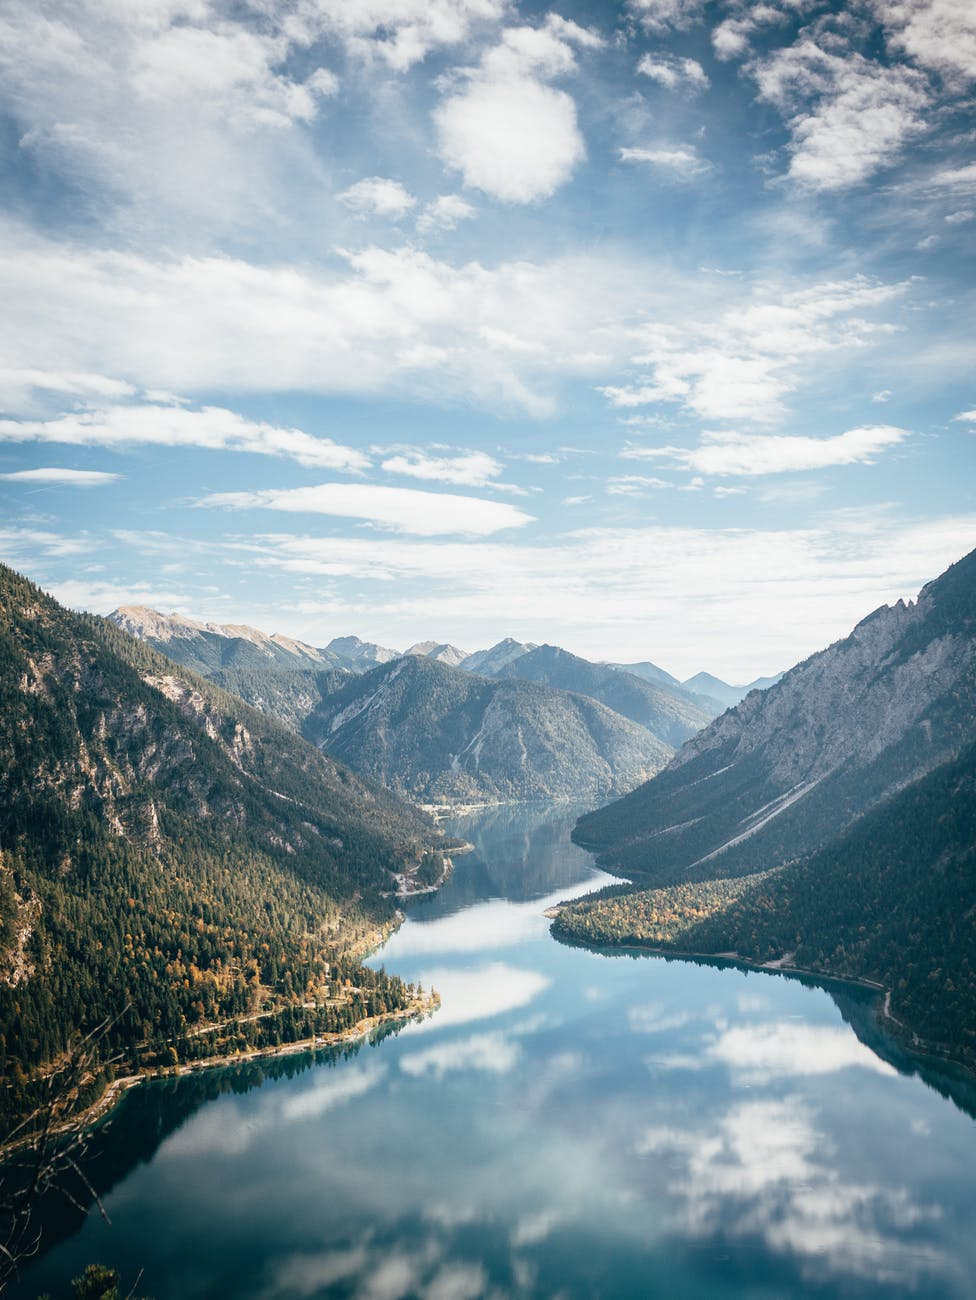
\includegraphics[width=0.49\columnwidth]{Figures/SampleImage-1}\label{SubFigure-1-label}}
\hfill
\subfloat[Sample Image 2 Caption]
{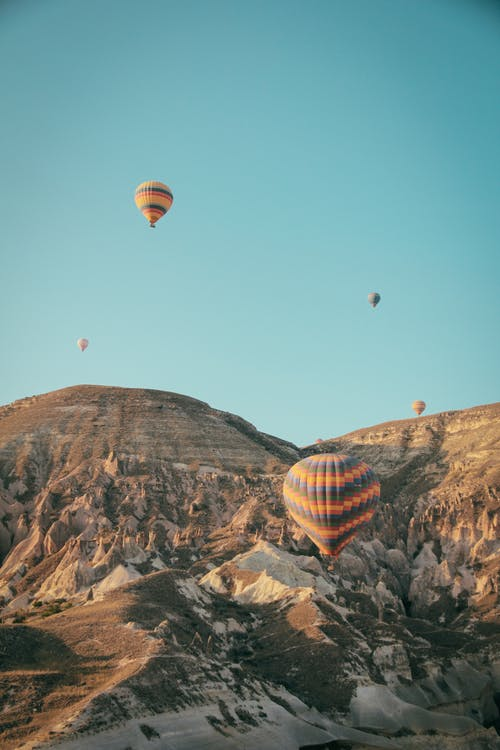
\includegraphics[width=0.49\columnwidth]{Figures/SampleImage-2}\label{SubFigure-2-label}}
\caption{Caption of Figure}
\label{FigureLabel}
\end{figure}

\newpage %Write table of contents of thesis from new page.
\section{PROPOSED CONTENTS OF THE THESIS}
\begin{enumerate}[labelwidth=2.4cm,labelindent=15pt,leftmargin=2.5cm,label=\bfseries CHAPTER \arabic*,align=left]
\setlength\itemsep{-0.2em}
%Start inserting contents from here
\item {\bf INTRODUCTION \rm}
\begin{itemize}[leftmargin=10pt]
\setlength\itemsep{-0.2em}
	\item[1.1]	PREAMBLE
	\item[1.2]	LITERATURE REVIEW
	\item[1.3]	OBJECTIVE AND SCOPE OF THE PRESENT RESEARCH WORK
	\item[1.4] 	ORGANIZATION OF THESIS 
\end{itemize}
\item {\bf CONCLUSIONS \rm}
\begin{itemize}[leftmargin=10pt]
	\item[2.1]	MAJOR CONTRIBUTIONS
	\item[2.2]	SCOPE FOR FUTURE WORK
\end{itemize}
\begin{itemize}[leftmargin=-2.5cm]
\setlength\itemsep{-0.2em}
\item[]{\bf REFERENCES \rm}
\item[]{\bf PUBLICATIONS FROM THIS THESIS \rm}
\end{itemize}
\end{enumerate}

\section{LIST OF PUBLICATIONS BASED ON THE RESEARCH WORK}
\subsection*{Patent Filed}
\begin{enumerate}
\item List patents if any else remove/comment this subsection.    
\end{enumerate}

\subsection*{Refereed Journals}
\begin{enumerate}
\item \textbf{Singh, S.}, \textbf{A. Roy} and \textbf{M.~P. Selvan} (2019) Smart load node for nonsmart load under smart grid paradigm: a new home energy management system. \textit{IEEE Consumer Electronics Magazine}, \textbf{8}(2), 22--27.
\end{enumerate}
\subsection*{International Conferences}
\begin{enumerate}
\item \textbf{Singh, S.}, \textbf{A. Namboodiri} and \textbf{M.~P. Selvan} (2019) Simplified algorithm for dynamic demand response in smart homes under smart grid environment. \textit{IEEE PES GTD Grand International Conference \& Exposition Asia}, Bangkok, Thailand.
\end{enumerate}

\subsection*{Papers Under Review}
\begin{enumerate}
\item Declare papers under review here (if needed). Otherwise you may delete/comment this subsection.
\end{enumerate}
\end{document} 